\documentclass[12pt]{amsart}
\usepackage[margin=1in, letterpaper]{geometry}
\usepackage[utf8]{inputenc}
\def\labelitemi{--}
\usepackage[english]{babel}
\usepackage{siunitx}
\usepackage{graphicx}
\graphicspath{ {./images/} }
\DeclareGraphicsExtensions{.pdf,.png,.jpg}
\usepackage{fancyhdr}
\usepackage{csquotes}
\usepackage{fixltx2e}
\setlength{\parskip}{11pt}
\setlength{\parindent}{0cm}
\usepackage{braket}
\usepackage{cancel}
\usepackage{hyperref}


%\defbeamertemplate{itemize item}{boldarrow}{\raisebox{0.3ex}{\resizebox{1.2ex}{1ex}{\ArrowBoldRightShort}}}

\usepackage{enumitem}
\newlist{arrowlist}{itemize}{1}
\setlist[arrowlist]{label=$\Rightarrow$}

\usepackage[utf8]{inputenc}
\usepackage{tikz}
\usetikzlibrary{shapes,arrows}
\usetikzlibrary{positioning}
\usetikzlibrary{backgrounds}

\usepackage{amsmath}
\DeclareMathOperator{\sech}{sech}
\DeclareMathOperator{\csch}{csch}
\DeclareMathOperator{\arcsec}{arcsec}
\DeclareMathOperator{\arccot}{arcCot}
\DeclareMathOperator{\arccsc}{arcCsc}
\DeclareMathOperator{\arccosh}{arcCosh}
\DeclareMathOperator{\arcsinh}{arcsinh}
\DeclareMathOperator{\arctanh}{arctanh}
\DeclareMathOperator{\arcsech}{arcsech}
\DeclareMathOperator{\arccsch}{arcCsch}
\DeclareMathOperator{\arccoth}{arcCoth}

\usepackage{caption}
\usepackage{subcaption}
% \captionof{table}{CAPTION}

\setlength{\tabcolsep}{6pt}
\renewcommand{\arraystretch}{1.2}
% \renewcommand{\arraystretch}{0.7} WHEN USING DOUBLE SPACING

\usepackage[utf8]{inputenc}
 
\usepackage{listings}
\usepackage{color}

\usepackage{courier}
\definecolor{codegreen}{rgb}{0,0.6,0}
\definecolor{codegray}{rgb}{0.5,0.5,0.5}
\definecolor{codepurple}{rgb}{0.58,0,0.82}
\definecolor{backcolour}{rgb}{0.95,0.95,0.92}
 
\lstdefinestyle{mystyle}{
    backgroundcolor=\color{backcolour},   
    commentstyle=\color{codegreen},
    keywordstyle=\color{magenta},
    numberstyle=\tiny\color{codegray},
    stringstyle=\color{codepurple},
    basicstyle=\footnotesize\ttfamily,
    breakatwhitespace=false,         
    breaklines=true,                 
    captionpos=b,                    
    keepspaces=true,                 
    numbers=left,                    
    numbersep=5pt,                  
    showspaces=false,                
    showstringspaces=false,
    showtabs=false,                  
    tabsize=2,
}
 
\lstset{style=mystyle}

\def\labelitemi{--}

\pagestyle{fancy}
\fancyhf{}
\fancyhead[L]{ \textsc{Operating Plan}}
\fancyhead[R]{\textsc{Machine Learning Team}}
\fancyfoot[LE,RO]{\thepage}

\fancypagestyle{firststyle}
{
\fancyhf{}
\fancyhead[C]{\textsc{Chemistry 121 Problem Set \#1}}
\fancyhead[L]{\textsc{Will Kent}}
\fancyhead[R]{\textsc{\today}}
\renewcommand{\headrulewidth}{0pt}
}

\usepackage[version=3]{mhchem}
\usepackage{siunitx}
\sisetup{detect-weight=true, detect-family=true} % Allows siunitx to be bold in text environment

\usepackage{array}
\usepackage{tabu}

\usepackage{multicol}

\usepackage{setspace}

\title{Operating Plan for Engineering Design Project}
\author{Will Kent, Jackson Dougherty, Keir Adams}
\date{\today}

\begin{document}

\maketitle





\section*{Project Schedule}

There are several principle steps to the project. We first need to finish work on image processing, thresholding, and contouring, so that we have the data to begin machine learning development and analysis. From there we will collect statistical information on all of the images available to the project, as well as research and develop machine learning methods to analyze the spray images. After developing the machine learning code, we will test it on the images while, concurrently, researching physical information that can be determined from the results of our machine learning analysis. This work should all be completed two to three weeks before the end of the project. Finally, we will use the machine learning methods developed to learn as much about the spray images available to the project and try to provide both quantitative and qualitative analysis on the performance of the spray nozzles. By this time we also will have packaged the code such that it will be easy for those who do not have programming experience to use and documented sufficiently for future software developers to modify and augment the project. Figure 1 illustrates this process and how all of the project nodes interact with on another.




\begin{figure}[h]
\begin{center}
% Define block styles
\tikzstyle{decision} = [diamond, draw, fill=green!20, 
    text width=4.5em, text badly centered, node distance=3cm, inner sep=0pt]
\tikzstyle{block} = [rectangle, draw, fill=blue!20, 
    text width=8em, text centered, rounded corners, minimum height=4em, node distance=2cm]
 \tikzstyle{gpio} = [rectangle, draw, fill=red!20, 
    text width=8em, text centered, rounded corners, minimum height=4em, node distance=2cm]
\tikzstyle{line} = [draw, -latex']
\tikzstyle{cloud} = [draw, ellipse,fill=red!20, node distance=3cm,
    minimum height=2em]
    
\begin{tikzpicture}[node distance = 2cm, auto]
    % Place nodes
    \node [gpio] (init) {Raw Images};
    \node [block, below of=init, node distance = 2.5cm] (kmeans) {$k$-means Clustering};
    \node [block, node distance=4cm, left of=kmeans] (filter) {Image Preprocessing};
    \node [block, node distance=4cm, right of=kmeans] (thresholding) {Thresholding and Contouring};
    \node [block, below of=kmeans, node distance = 2.9cm] (stat) {Conventional Statistical Analysis};
    \node [block, node distance=4cm, left of=stat] (grouping) {Shape Grouping};
     \node [block, node distance=4cm, right of=stat] (cdata) {Create Training Data};
     \node [gpio, node distance=2.5cm, below of=stat] (tdata) {Training Data};
     \node [block, node distance=2.5cm, below of=tdata] (time) {Frame Tracking};
      \node [block, node distance=4cm, left of=time] (ml) {Machine Learning Analysis};
      \node [block, node distance=4cm, right of=time] (flow) {Flow/Atomization Characterization};
     \node [gpio] (tml) at (-2,-13) {Trained ML Algorithm};
     \node [gpio] (pinfo) at (2,-13) {Characterization of Spray};
    % Draw lines
    \path [line] (init) -- (0,-1.3);
    \begin{scope}[on background layer]
   	 \filldraw [fill=gray!20, rounded corners, line width=1pt] (0,-1.3) -- (6.15,-1.3) -- (6.15,-3.7) -- (-6.15,-3.7) -- (-6.15,-1.3) -- (0,-1.3);
    \end{scope}
    \path [line] (-6.15,-2.5) -- (filter);
    \path [line] (filter) -- (kmeans);
    \path [line] (kmeans) -- (thresholding);
    \path [line] (thresholding) -- (6.15,-2.5); 
    \path [line] (0,-3.7) -- (0,-4.2);
    \begin{scope}[on background layer]
   	 \filldraw [fill=gray!20, rounded corners, line width=1pt] (0,-4.2) -- (6.15,-4.2) -- (6.15,-6.6) -- (-6.15,-6.6) -- (-6.15,-4.2) -- (0,-4.2);
    \end{scope}
     \path [line] (-6.15,-5.4) -- (grouping);
    \path [line] (grouping) -- (stat);
    \path [line] (stat) -- (cdata);
    \path [line] (cdata) -- (6.15,-5.4); 
    \path [line] (0,-6.6) -- (0,-7.1);
    \path [line] (tdata) -- (0,-9.2);
    \begin{scope}[on background layer]
   	 \filldraw [fill=gray!20, rounded corners, line width=1pt] (0,-9.2) -- (6.15,-9.2) -- (6.15,-11.6) -- (-6.15,-11.6) -- (-6.15,-9.2) -- (0,-9.2);
    \end{scope}
    \path [line] (-6.15,-10.4) -- (ml);
    \path [line] (ml) -- (time);
    \path [line] (time) -- (flow);
    \path [line] (flow) -- (6.15,-10.4); 
    \path [line] (ml) -- (-4,-11.6);
     \path [line] (time) -- (0,-11.6);
      \path [line] (flow) -- (4,-11.6);
     \path [line] (-2,-11.6) -- (tml);
      \path [line] (2,-11.6) -- (pinfo);
\end{tikzpicture}
\end{center}
\captionof{figure}{Project flow: blue nodes are processes or functions, red nodes are outputs and/or inputs}
\end{figure}


Below you will find a week by week schedule on how the project will proceed. It outlines week by week what the team will accomplish, as well as deadlines for key materials like presentations and reports. In addition to the weekly tasks mentioned in the below schedule, the design team will meet with Xiaoying Liu one to two times a week, and meet with external mentors at a frequency to be determined. 

\begin{center}
\textbf{Autumn}
\end{center}

Week 4
\vspace*{-11pt}
\begin{itemize}
	\item Deadline: Draft of SOW and OP
	\item Finish thresholding work
	\item Get details on cloud file storage
	\item Crop all images to prevent background noise 
	\item Meet with Doug MacAuley on Monday
	\item Contact external mentors
	\item Deadline: Finalized SOW and OP, presentation of OP to Xiaoying (5min)
	\item Revise SOW and OP based upon feedback from mentors and Xiaoying
\end{itemize}

Week 5
\vspace*{-11pt}
\begin{itemize}
	\item Investigate \textit{openCV} methods for collecting information on shape, size, density (color), position, and time distribution of droplets
	\item Generate statistical information, namely distributions of information mentioned in previous bullitt point.
\end{itemize}

Week 6
\vspace*{-11pt}
\begin{itemize}
	\item Complete droplet cataloging and analysis from week 5
	\item Commence research on machine learning methods
	\begin{itemize}
		\item Keir: neural networks, ridge regression
		\item Will: Random forest walk and other unsupervised methods
		\item Jackson: Support vector machines, genetic algorithms
	\end{itemize}
\end{itemize}

Week 7
\vspace*{-11pt}
\begin{itemize}
	\item Decide on most promising machine learning methods to pursue
	\item Create python frameworks for each method (see Figure 1 \textbf{Machine Learning})
	\item Start researching frame tracking and temporal data collection
	\item Start researching physical information to track 
\end{itemize}

Week 8
\vspace*{-11pt}
\begin{itemize}
	\item Hyper-parameter optimization
	\item Continue research into physical information for tracking
	\item Continue researching frame tracking and temporal data collection
\end{itemize}

Week 9
\vspace*{-11pt}
\begin{itemize}
	\item Continue hyper-parameter optimization
	\item Continue research into physical information for tracking
	\item Develop and code frame tracking and temporal data collection
	\item Begin working on mid-project presentation and progress report
\end{itemize}

Week 10
\vspace*{-11pt}
\begin{itemize}
	\item Finish hyper-parameter optimization
	\item Continue research into physical information for tracking
	\item Develop and code frame tracking and temporal data collection
	\item Present mid-project presentation 
	\item Finish progress report
\end{itemize}

Week 11
\vspace*{-11pt}
\begin{itemize}
	\item Revise mid-project presentation based on class feedback
	\item Present progress report and mid-project presentation to external mentor
\end{itemize}

\begin{center}
\textbf{Winter}
\end{center}

Week1
\vspace*{-11pt}
\begin{itemize}
	\item Continue research into physical information for tracking
	\item Continue development and coding of frame tracking and temporal data collection
\end{itemize}

Week 2
\vspace*{-11pt}
\begin{itemize}
	\item Continue research into physical information for tracking
	\item Continue development and coding of frame tracking and temporal data collection
	\item Augment machine learning methods to accommodate frame tracking and physical information
\end{itemize}

Week 3
\vspace*{-11pt}
\begin{itemize}
	\item Present progress report to external mentor
	\item Continue research into physical information for tracking
	\item Finish development and coding of frame tracking and temporal data collection
	\item Test code for frame tracking and temporal data collection
	\item Continue augmenting machine learning methods to accommodate frame tracking and physical information
\end{itemize}

Week 4
\vspace*{-11pt}
\begin{itemize}
	\item Finish research into physical information for tracking
	\item Improve and continue to test frame tracking and temporal data collection code
	\item Continue augmenting machine learning methods to accommodate frame tracking and physical information
	\item Prepare mid-quarter presentation to the mentors
\end{itemize}

Week 5
\vspace*{-11pt}
\begin{itemize}
	\item Continue improving and testing code for frame tracking and temporal data 
	\item Test physical information tracking code
	\item Present mid-quarter presentation to the mentors
\end{itemize}

Week 6 
\vspace*{-11pt}
\begin{itemize}
	\item Continue improving and testing code for frame tracking and temporal data 
	\item Improve and continue to test physical information tracking code
\end{itemize}

Week 7
\vspace*{-11pt}
\begin{itemize}
	\item Finalize code for frame tracking and temporal data 
	\item Finalize physical information tracking code
	\item Begin packaging project for ease-of-use and further development 
	\item Begin final analysis of provided spray data
\end{itemize}

Week 8
\vspace*{-11pt}
\begin{itemize}
	\item Finish final analysis of provided spray data 
	\item Finish packaging project for ease-of-use and further development
	\item Begin final report for design project
\end{itemize}

Week 9
\vspace*{-11pt}
\begin{itemize}
	\item Continue work on final report for design project
	\item Prepare final presentation to the class
\end{itemize}

Week 10:
\vspace*{-11pt}
\begin{itemize}
	\item Complete design project
	\item Finish final report 
	\item Deadline: present final presentation to the class
\end{itemize}

Week 11:
\vspace*{-11pt}
\begin{itemize}
	\item Deadline: final report and presentations to external mentors
\end{itemize}






\section*{Organization of Project Materials}

Both for the project to proceed efficiently and for the project to continue after the allotted two quarter timespan, the code and documents need to be organized effectively and the project materials must be documented effectively. There are three main structures that we have mapped: what the final project should do, what files will be included and how they will interact with one another, and how the files will be stored. Previous sections have outline what the project will accomplish and how the different portions of the project will interact with each other (see Figure 1 and $\ldots$). Now we will examine \textit{how} the different portions of the project will be actualized and organized. 

As should be clear from the discussions of image thresholding, clustering, and machine learning algorithms, there are many different moving parts to this project. Multiple programming libraries will be used to generate plots, statistical information, machine learning settings, as well as many outputs. The heterogeneity of the different sections of the project and the fact that three programmers will be working on the same code at a given time requires a highly coordinated effort. If the group is not coordinated, it will be difficult to test code, combine work from multiple individuals, and finish the project in a manner that allows for further development. To prevent these undesirable outcomes, we have outlined two structures: what kinds of program files will be present and how they will interact with one another, and where files will be stored and how they will be organized. 

It was decided amongst the group to code the project entirely in Python because of the access to machine learning libraries that it proves as well as the common basis everyone in the team shares. \textsc{Figure 2} shows the different kinds of files that will be used and how they will interact with one another. The ultimate goal of the project is to develop the code rigorously enough to the point where a user will only need to specify the address of files in an input/parameters file (colored yellow in \textsc{Figure 2}) and execute a python file (\textit{run.py}) to run analysis on image files. This run file will read information from the input file, find the images, create directories for output, and then pass all of the necessary information to another file (\textit{run\_analysis}) that will run analysis on the images. We will call these files \textit{execution files} (see (2) in \textsc{Figure 2}).

The analysis file will call upon functions from several \textit{main files}. These files include the programs for $k$-means cluster analysis and thresholding, documentation of results and settings, image processing, and machine learning (see (3) in \textsc{Figure 2}). The programs within the \textit{main files} will call upon functions written in $\textit{auxiliary files}$. These auxiliary files will include process specific auxiliary files, such as \textit{thresholding\_aux.py} or \textit{ML1\_aux.py}, but also contain files with more general functions, such as reading and writing images into files, plotting images, and documenting results. This structure is important because using \textit{auxiliary files} will allow the \textit{main files} to be coded in fewer lines and begin at the top of the files. This will make the code easier to debug, documents, and significantly easier to follow both for team members and any future developers. The \textit{auxiliary files} will also include python files for every single instance of plots, so that plots from every part of the project can be automatically regenerated if on node in the project is changed significantly. Finally, personal development files for each developer will be within the auxiliary files so that developers can test code before adding it to the project functions and potentially damaging other work on the project. 


% Define block styles
\tikzstyle{repo} = [rectangle, draw, fill=orange!30, 
    text width=6em, text badly centered, rounded corners, minimum height=4em, minimum width = 9em, node distance=5cm, inner sep=0pt, line width = 1pt]
    \tikzstyle{comp} = [rectangle, draw, fill=gray!20, 
    text width=6em, text badly centered, rounded corners, minimum height=4em, minimum width = 9em, node distance=5cm, inner sep=0pt, line width = 1pt]
\tikzstyle{python} = [rectangle, draw, fill=green!30,
    text width=4.5em, text badly centered,  minimum height=4em, minimum width = 9em, rounded corners, node distance=5cm, inner sep=0pt]
\tikzstyle{notpy} = [rectangle, draw, fill=yellow!30, 
    text width=8em, text centered, rounded corners, minimum height=4em, node distance=2cm, minimum width=9em]
 \tikzstyle{file} = [rectangle, draw, fill=red!30, 
    text width=8em, text centered, rounded corners, minimum height=4em, node distance=2cm]
\tikzstyle{line} = [draw, -latex']

\begin{figure}[h]
\begin{center}
\begin{tikzpicture}[node distance = 2cm, auto]
    % Place nodes
    \node [repo] (init) {\textbf{Git Repository}};
    \node [comp, left of=init] (personal) {\textbf{Personal Computers}};
    \node [comp, right of=init] (hep) {\textbf{HEP Bld. Computers}};
    \node [python, below of=init, node distance=2.5cm, text width=2cm] (run) {\textit{run.py}};
    \node [python, right of=run, node distance=5cm, text width=3cm] (runanalysis) {\textit{run\_analysis.py}};
    \node [notpy, left of=run, node distance=5cm, text width=3cm] (input) {\textbf{Inputs and Parameters} \textit{params.json/.txt}};
     \node [python, below of=run, node distance=4cm, text width=3.25cm, minimum height = 9em] (ml) {\textbf{Machine Learning}  \textit{MLmethod1.py} \textit{MLmethod2.py} \textit{MLmethod2.py} $\ldots$ \textit{MLmethodN.py}};
      \node [python, left of=ml, node distance=5cm, minimum height = 9em, text width=3cm] (kmth) {\textbf{k-means + Thresholding} \textit{thresholding.py}  \textit{kmeans.py}};
      \node [python, below of=runanalysis, node distance=3cm, minimum height = 4em, text width=3cm] (doc) {\textbf{Documentation} \textit{documenting.py}};
       \node [python, below of=doc, node distance=2cm, minimum height = 4em, text width=3cm] (filter) {\textbf{Image Processing} \textit{preprocess.py}};
       \node [python, below of=kmth, node distance=4.2cm, minimum height = 7em, text width=3cm] (gpio) {\textbf{Reading/ Writing Files} \textit{readimage.py} \textit{writeimage.py} \textit{savesettings.py}};
       \node [python, below of=ml, node distance=5cm, minimum height = 11em, text width=4cm] (aux) {\textbf{Auxiliary Functions} \textit{thresholding\_aux.py} \textit{preprocess\_aux.py} \textit{kmeans\_aux.py} \textit{ML1\_aux.py} $\ldots$ \textit{MLN\_aux.py} \textit{documenting\_aux.py}};
         \node [python, below of=filter, node distance=3cm, minimum height = 6em, text width=3cm] (dev) {\textbf{Individual Developers} \textit{will.py} \textit{keir.py} \textit{jackson.py} };
         \node [python, below of=dev, node distance=2.45cm, minimum height = 4em, text width=3cm] (plot) {\textbf{Plotting Functions} \textit{plotting.py}};
         \node [python, below of=gpio, node distance=3.3cm, minimum height = 7em, text width=3cm] (plots) {\textbf{Plotting Files} \textit{prepro\_plots.py} \textit{kmeans\_plots.py} \textit{thres\_plots.py} \textit{ML1\_plots.py}};
    % Draw edges
    \draw [line width = 1pt] (init) -- (0, -1.03) ;
    \begin{scope}[on background layer]
   	 \filldraw [fill=blue!10, rounded corners, line width=1pt] (0, -1.03) -- (-8.5,-1.35) -- (-8.5,-16)--(8.5,-16)--(8.5,-1.35) -- (0,-1.03);
    \end{scope}
    \path [line] (run) -- (runanalysis);
     \path [line] (input) -- (run);
    \path [line] (ml) -- (0,-4) -- (5,-4) -- (5,-3.3);
    \path [line] (kmth) -- (-5,-3.75) -- (4.75,-3.75) -- (4.75,-3.3);
    \path [line] (kmth) -- (-2.5,-6.5)  -- (-2.5,-14.5) -- (-3.1,-14.5);
    \path [line] (doc) -- (5,-4.65) -- (5.5,-4.25) -- (5.5,-3.3);
    \draw [line] (filter) -- (2.5,-7.5) -- (2.5,-4.45) -- (5,-4.45) -- (5.25,-4.25) -- (5.25,-3.3);
    \draw [line] (filter) -- (7.5,-7.5) -- (7.5,-14.75) -- (-3.1,-14.75);
    \path [line]  (gpio) -- (kmth);
    \path [line] (gpio) -- (-5.25,-9.25) -- (-5.25,-8.9) -- (-0.25,-8.9) -- (-0.25,-8.36);
    \path [line] (gpio) -- (-4.75,-9.25) -- (-4.75,-8.8) -- (4.75,-8.8) -- (4.75,-8.36);
   \path [line] (gpio) -- (-5.5,-9.25) -- (-5.5,-8.9) -- (-8,-8.9) -- (-8,-15.7) -- (8.25,-15.7) -- (8.25,-5.5) -- (6.9,-5.5);
   \path [line] (gpio) -- (-5.75,-9.25) -- (-5.75,-8.8) -- (-8,-8.8) -- (-8,-4.25) -- (4.5,-4.25) -- (4.5,-3.3) ;
    \path [line] (aux) -- (ml);
    \path [line] (aux) -- (-0.5,-9.2) -- (-0.5,-8.7) -- (-0.5,-8.7) -- (-4.75,-8.7)-- (-4.75,-8.36);
   \path [line] (aux) -- (0.5,-9.2) -- (0.5,-8.7) -- (4.5,-8.7) -- (4.5,-8.36);
   \path [line] (dev) -- (filter);
   \path [line] (dev) -- (4,-9.25) -- (4,-8.9) -- (1.5,-8.9) -- (1.5,-8.6) -- (-5.25,-8.6) -- (-5.25,-8.36);
    \path [line] (dev) -- (4.25,-9.25) -- (4.25,-8.5) -- (0.5,-8.5) -- (0.5,-8.36);
    \path [line] (plot) -- (2.5,-12.95) -- (2.5,-9.10) --  (0.25,-9.10) -- (0.25,-8.36);
    \path [line] (plot) -- (2.5,-12.95) -- (2.5,-9) --  (5.25,-9) -- (5.25,-8.34);
    \path [line] (plot) -- (2.5,-12.95) -- (2.5,-9) -- (-4.5,-9) -- (-4.5,-8.36);
    \path [line] (plot) -- (5,-15) -- (-3.1,-15) ; 
    \path [line] (ml) -- (-2.5,-6.5) -- (-2.5,-14.5) -- (-3.1,-14.5);
    \path [line] (gpio) -- (plots);
    \path [line] (dev)  -- (8,-10.5) -- (8,-15.25) -- (-3.1,-15.25);
    \path [line, line width = 1pt] (init) -- (personal);
    \path [line, line width = 1pt] (init) -- (hep);
    \path [line, line width = 1pt] (hep) -- (init);
    \path [line, line width = 1pt] (personal) -- (init);
    \draw [line width = 1pt] (9,1) -- node {(1)} (9,-1);
    \draw [line width = 1pt] (8.8,1) -- (9.2,1);
    \draw [line width = 1pt] (8.8,-1) -- (9.2,-1);
    \draw [line width = 1pt] (9,-1.5) -- node {(2)} (9,-3.5);
     \draw [line width = 1pt] (8.8,-1.5) -- (9.2,-1.5);
    \draw [line width = 1pt] (8.8,-3.5) -- (9.2,-3.5);
    \draw [line width = 1pt] (9,-4.5) -- node {(3)} (9,-8.5);
     \draw [line width = 1pt] (8.8,-4.5) -- (9.2,-4.5);
    \draw [line width = 1pt] (8.8,-8.5) -- (9.2,-8.5);
    \draw [line width = 1pt] (9,-9) -- node {(4)} (9,-15.7);
     \draw [line width = 1pt] (8.8,-9) -- (9.2,-9);
    \draw [line width = 1pt] (8.8,-15.7) -- (9.2,-15.7);
\end{tikzpicture}
\end{center}
\captionof{figure}{Code Structure: (1) Computers/storage (2) Execution Files (3) Main Files (4) Auxiliary Files. Each green node is a python file or a group of python files.}
\end{figure}

In order to facilitate working on the project with multiple software developers, we will use git, an open source distributed version control system, and host the project code on GitHub, a cloud-based git repository. The repository is called \texttt{MENGEDML} and can be checked out at the address \url{https://github.com/wkent2020/MENGEDML.git}. Using git will allow the team to share work and keep detailed track of each change to the master code (see \textsc{Figure 3}). In addition to keeping track of all changes to the code, git allows for all of the team to develop code on their personal computers and test it on other devices. 

\begin{figure}[h]
\begin{center}
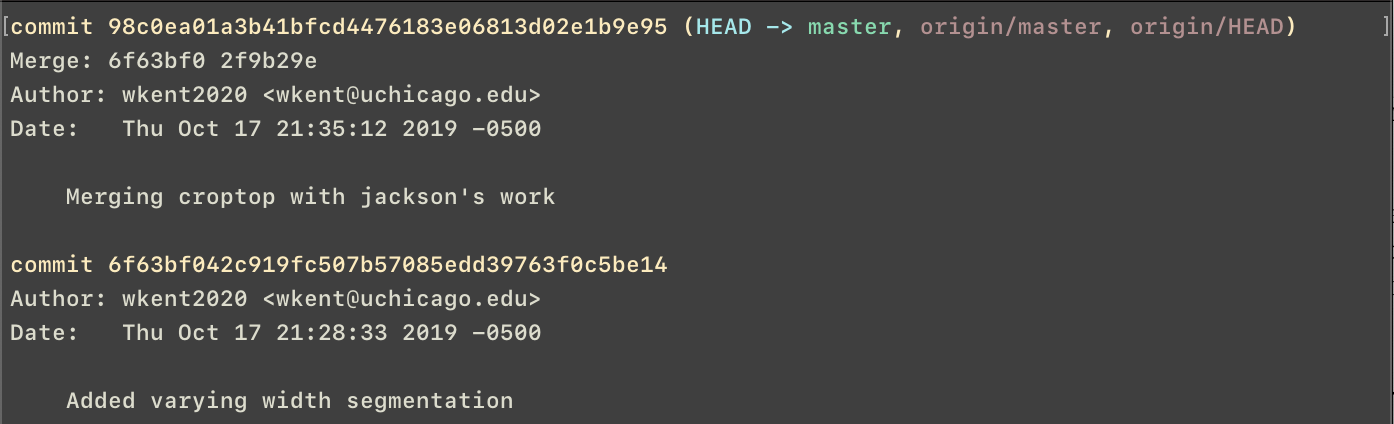
\includegraphics[width=6in]{1.png}
\captionof{figure}{Example git log: git keeps track of every change made to the code, who made the change, and allows users to revert to past version. }
\end{center}
\end{figure}

One problem facing the project is how files will be \textit{stored} and \textit{where} they will be stored. The files within the git repository will be organized as follows:

\begin{multicols}{2}
Git Repository
\vspace*{-11pt}
\begin{itemize}
	\item[] \textit{kmeans\_thesh.py}
	\item[] \textit{preprocess.py}
	\item[] \textit{documenting.py}
	\item[] \textit{plotting.py}
	\item[] \textit{run.py}
	\item[] \textit{run\_analysis.py}
	\item[] \textit{params.json/.txt}
	\item[]  $\vdots$
	\item[]  \textit{mainN.py}
	\item[$\Rightarrow$] Auxiliary Functions [Auxiliary Functions Files]
		\begin{itemize}
			\item[] \textit{thesholding\_aux.py}
			\item[] \textit{kmeans\_aux.py}
			\item[] \textit{preprocess\_aux.py}
			\item[] $\vdots$
		\end{itemize}
	\item[$\Rightarrow$] Plotting [Plotting files and Data]
		\begin{itemize}
			\item[] \textit{plotting.py}
			\item[] \textit{kmeans\_plotting.py}
			\item[] \textit{preprocess\_plotting.py}
			\item[] $\vdots$
			\item[$\Rightarrow$] Plots
			\begin{itemize}
				\item[$\Rightarrow$] Thresholding Plots
				\item[$\Rightarrow$] Pre Processed Images
				\item[$\Rightarrow$] ML Method 1 Plots
			\end{itemize}
		\end{itemize}
	\item[$\Rightarrow$] Documentation
			\begin{itemize}
				\item[$\Rightarrow$] K-means Docs
				\item[$\Rightarrow$] ML Docs
				\item[$\Rightarrow$] Papers
				\item[$\Rightarrow$] Plotting Docs
			\end{itemize}
	\item[$\Rightarrow$] Individual
		\begin{itemize}
			\item[] \textit{will.py}
			\item[] \textit{keir.py}
			\item[] \textit{jackson.py}
		\end{itemize}
\end{itemize}
\end{multicols}

Because of the available images files are so numerous, we cannot store the team cannot store them on personal computers. Thus, we will store image files on two desktops located in the High Energy Physics Building which can be accessed remotely. 

\section*{Conclusion}

We have outlined the goals, focuses, organization, and schedule for our design project. We will develop tools for evaluating droplet structure and spatial spray distribution, construct a coding framework for researchers, and evaluate the performance of the fuel injection technology examined during our project. Clustering algorithms and image contouring software will be used to curate data for training machine learning algorithms. These intelligent analytical methods will be used to identify features and trends in fuel injection sprays otherwise imperceptible to the human eye and conventional methods of statistical analysis. After constructing and testing all of these tools, we will evaluate the performance of the provided spray information. By the conclusion of our design project, we will have produced an accessible tool for evaluating the performance of fuel injection technology. 




\end{document}